
% -- coding: UTF-8 -- 

% This is a simple template for a LaTeX document using the "article" class.
% See "book", "report", "letter" for other types of document.

\documentclass[a4paper,11pt,UTF8]{ctexart}

%%% Examples of Article customizations
% These packages are optional, depending whether you want the features they provide.
% See the LaTeX Companion or other references for full information.

%%% PAGE DIMENSIONS
\usepackage{geometry} % to change the page dimensions
\geometry{top=3cm,bottom=3cm}
%\geometry{margin=1.4in} % for example, change the margins to 2 inches all round
% \geometry{landscape} % set up the page for landscape
%   read geometry.pdf for detailed page layout information

\usepackage{graphicx} % support the \includegraphics command and options
\usepackage{amsmath}
\newcommand{\upcite}[1]{\textsuperscript{\textsuperscript{\cite{#1}}}}
% \usepackage[parfill]{parskip} % Activate to begin paragraphs with an empty line rather than an indent
\usepackage[titletoc]{appendix}
\usepackage{listings}
\usepackage{color}

\definecolor{dkgreen}{rgb}{0,0.6,0}
\definecolor{gray}{rgb}{0.5,0.5,0.5}
\definecolor{mauve}{rgb}{0.58,0,0.82}

\lstset{frame=tb,
  language=C++,
  aboveskip=3mm,
  belowskip=3mm,
  showstringspaces=false,
  columns=flexible,
  basicstyle={\small\ttfamily},
  numbers=none,
  numberstyle=\tiny\color{gray},
  keywordstyle=\color{blue},
  commentstyle=\color{dkgreen},
  stringstyle=\color{mauve},
  breaklines=true,
  breakatwhitespace=true,
  tabsize=3
}
%%% PACKAGES
%\usepackage{booktabs} % for much better looking tables
%\usepackage{array} % for better arrays (eg matrices) in maths
%\usepackage{paralist} % very flexible & customisable lists (eg. enumerate/itemize, etc.)
%\usepackage{verbatim} % adds environment for commenting out blocks of text & for better verbatim
%\usepackage{subfig} % make it possible to include more than one captioned figure/table in a single float
% These packages are all incorporated in the memoir class to one degree or another...

%%% HEADERS & FOOTERS
%\usepackage{fancyhdr} % This should be set AFTER setting up the page geometry
%\pagestyle{fancy} % options: empty , plain , fancy
%\renewcommand{\headrulewidth}{0pt} % customise the layout...
%\lhead{}\chead{}\rhead{}
%\lfoot{}\cfoot{\thepage}\rfoot{}

%%% SECTION TITLE APPEARANCE
%\usepackage{sectsty}
%\allsectionsfont{\sffamily\mdseries\upshape} % (See the fntguide.pdf for font help)
% (This matches ConTeXt defaults)

%%% ToC (table of contents) APPEARANCE
%\usepackage[nottoc,notlof,notlot]{tocbibind} % Put the bibliography in the ToC
%\usepackage[titles,subfigure]{tocloft} % Alter the style of the Table of Contents
%\renewcommand{\cftsecfont}{\rmfamily\mdseries\upshape}
%\renewcommand{\cftsecpagefont}{\rmfamily\mdseries\upshape} % No bold!
%%% END Article customizations

%%% The "real" document content comes below...

\begin{document}

\title{可视化与可视计算概论第一次作业报告}
\author{1700012764 陈智斌}
%\date{} % Activate to display a given date or no date (if empty),
         % otherwise the current date is printed 

\maketitle
\tableofcontents

\newpage

\section{作业要求}

本次作业要求从NSFC资助项目统计资料中选取不少于三张有联系的表单,分别使用D3.js对各表单进行可视化,组成一个完整的可视化页面。在该份作业中,选择了以下三张表单:

1.2018年面上项目按申请与资助情况统计;

2.2018年面上项目资助情况(按单位隶属关系统计);

3.2018年面上项目资助情况(按单位性质统计);

\section{数据描述与分析}

\subsection{按申请与资助情况统计}

\begin{figure}[ht]
\centering
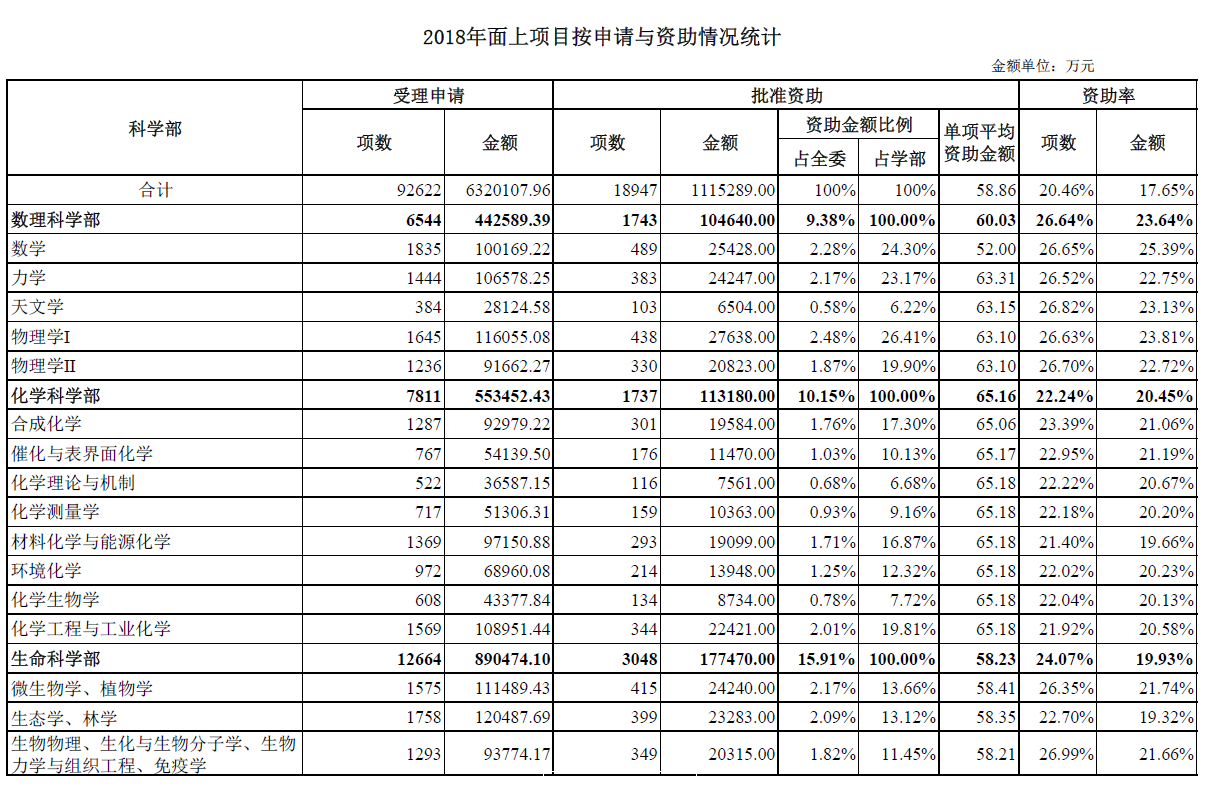
\includegraphics[scale=0.25]{QQ20191028140117.png}
\caption{表单1总览}
\end{figure}

这份数据按照科学部与进一步细分的一级学科为分类,记录了受理项目数、受理金额、批准资助项目数、批准金额及其占比、单项平均资助金额、资助率,其中从受理项目数、受理金额、批准资助项目数、批准金额出发,经过计算可以得到其他所有数据特征。如果以各一级学科为基础分类,该表单共计有学科、受理申请项数、受理金额、批准资助项数、批准金额、资助金额占全委比例、资助金额占学部比例、单项平均资助金额、资助项数率、资助金额率共计十个维度的数据,其中后五个维度数据可以由前五个维度推导而来,共计有8个科学部、55个一级学科。考虑期单项平均资助金额、资助率大多相近,可视化应主要考虑体现前五个维度的数据,同时适当体现资助金额比例之间的关系,单项平均资助金额、资助率可以通过一些显性的数值计算、几何比例体现。

\subsection{按单位隶属关系统计}

\begin{figure}[ht]
\centering
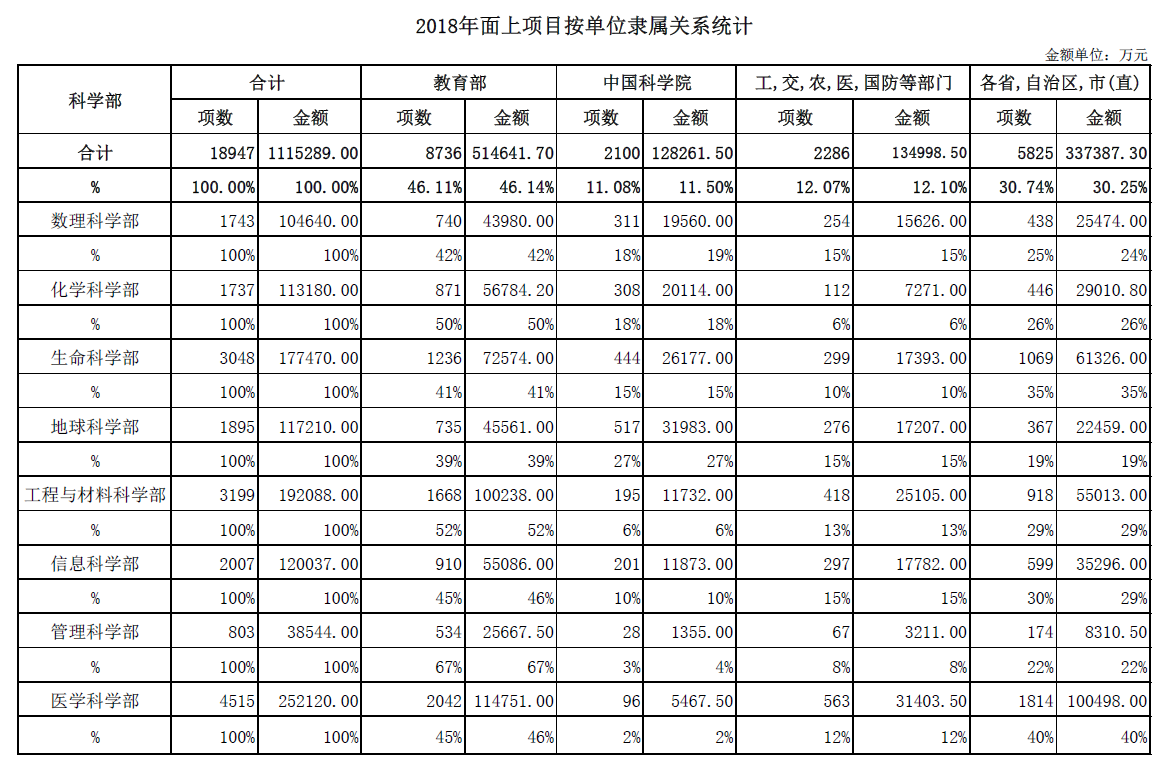
\includegraphics[scale=0.25]{QQ20191028141521.png}
\caption{表单2总览}
\end{figure}

这份数据按照科学部为分类,记录了批准的总项数、总金额,教育部、中国科学院、公交农医国防部门、省市自治区四种单位隶属关系各自的批准项数、批准金额及其所占比例。该表单共计有科学部、总项数、总金额、四种隶属关系每种的项数及比例、金额及比例,共计19个维度的数据,其中各项比例可以推导得来。该表单中各科学部、各部门比例差距较大,可以比较好地展现出各科学部发展与不同隶属单位之间的关系,因此各维度数据都较为重要,并集中分析各比例之间的关系。

\subsection{按单位性质统计}

\begin{figure}[ht]
\centering
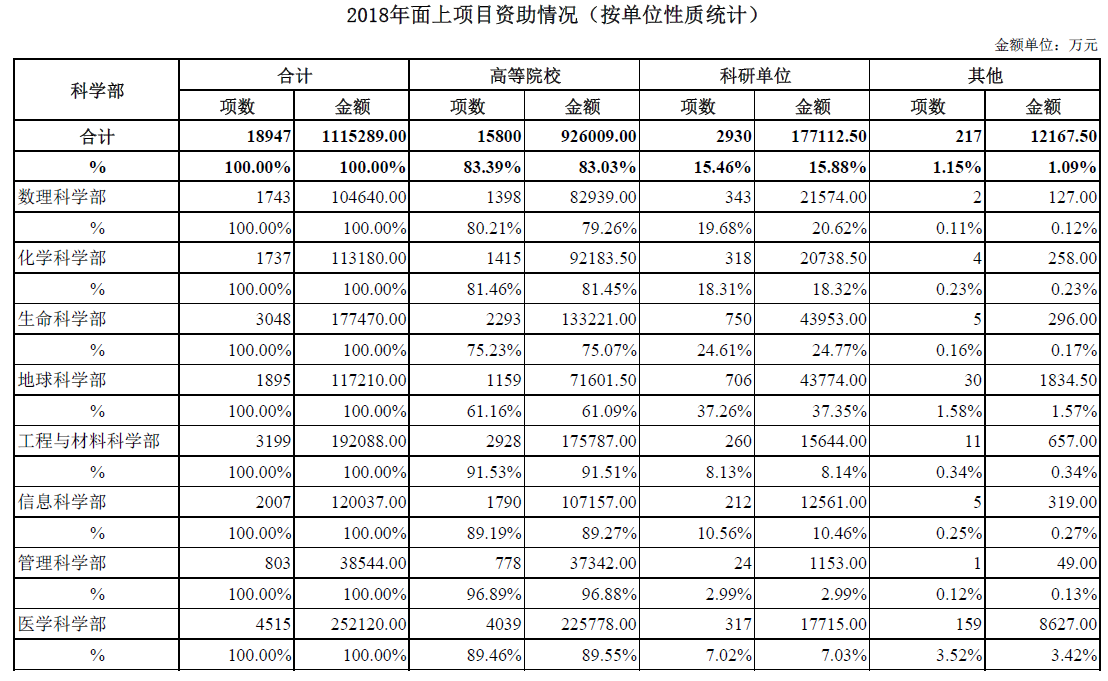
\includegraphics[scale=0.25]{QQ20191028142943.png}
\caption{表单3总览}
\end{figure}

这份数据按照科学部为分类,记录了批准的总项数、总金额,高等院校、科研单位、其他单位三种单位性质的各自的批准项数、批准金额及其所占比例。该表单共计有科学部、总项数、总金额、三种单位性质每种的项数及比例、金额及比例,共计15个维度的数据,其中各项比例可以推导得来。与第二张表单类似,由于各种比例差距较大,应当集中分析各比例之间的关系。

\section{设计宗旨和设计过程}

\subsection{表单1}

对这个表单可视化的关注点应该着重体现资助金额、资助项数之间的数量关系,以直观地表达出各科学部、各一级学科之间发展的差异、资助投入力度的大小。考虑使用柱状图来进行数据的可视化,以金额、项数为纵轴,以科学部、一级学科为横轴,为了直观、方便地比较科学部、一级学科之间的数量关系,分别以两种分类标准进行两张图的可视化绘制。

柱状图方法的好处是可以大体直观地体现数量关系,但难点在于无法体现维数过高的数据,进而无法将所有精确比例直接展现出来,因此考虑辅以标签、文字来进行可视化。

\subsection{表单2、3}

这两张表单情况比较类似,都应该着重体现各个比例之间的数量关系,以直观地表现出不同科学部在不同隶属关系、不同单位性质下的资助差异、发展程度。由于需要体现的维数较高。考虑使用平行坐标轴图来进行数据的可视化,每个维度各自使用一个坐标轴。

平行坐标轴图可以方便地容纳高维数的数据、体现数据之间的大小关系,但难点在于各数据之间的绝对倍率关系体现不直观,且实现难度较大。

\subsection{可视化页面}

从上面的设计过程可以知道,整个可视化页面将由四张可视化图像组成,故考虑在页面内部使用2*2排布方式,以方便在各个可视化图像之间进行比较、关联,并且易于与可视化图像进行交互,但不足之处在于页面整体本身没有装饰、结构较为简单。

\section{结果描述}

\subsection{表单1}

\begin{figure}[h]
\centering
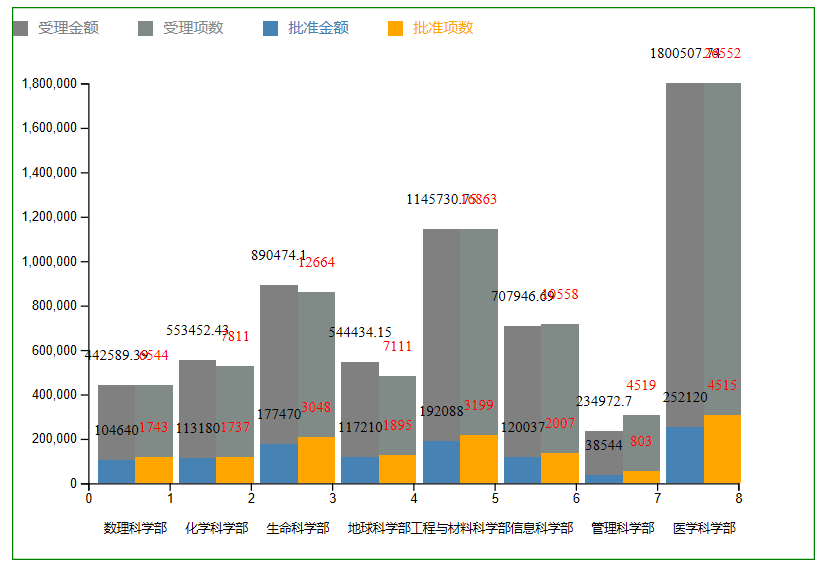
\includegraphics[scale=0.4]{QQ20191028155318.png}
\caption{表单1 以科学部为分类标准的可视化}
\end{figure}

以科学部为分类标准,总共有8类。每一类都有受理申请项数、受理申请金额、批准项数、批准金额,分别用两种灰色及橘色、蓝色表示,在横轴上标出每个类别的名字,在柱状图上标出各类的精确数值。从图上可以直观地看出,医学科学部不论是申请项数还是申请金额都超过了其他所有的科学部,说明该资助项目在医学方向投入的资助量是最大的,而管理科学部的申请项数和申请金额都是最少的。此外,从该图中可以看除,项数和资助金额基本上是成正相关的,批准金额和受理申请金额也是正相关的,这说明资助项目的供需关系基本是比较稳定的。

\begin{figure}[h]
\centering
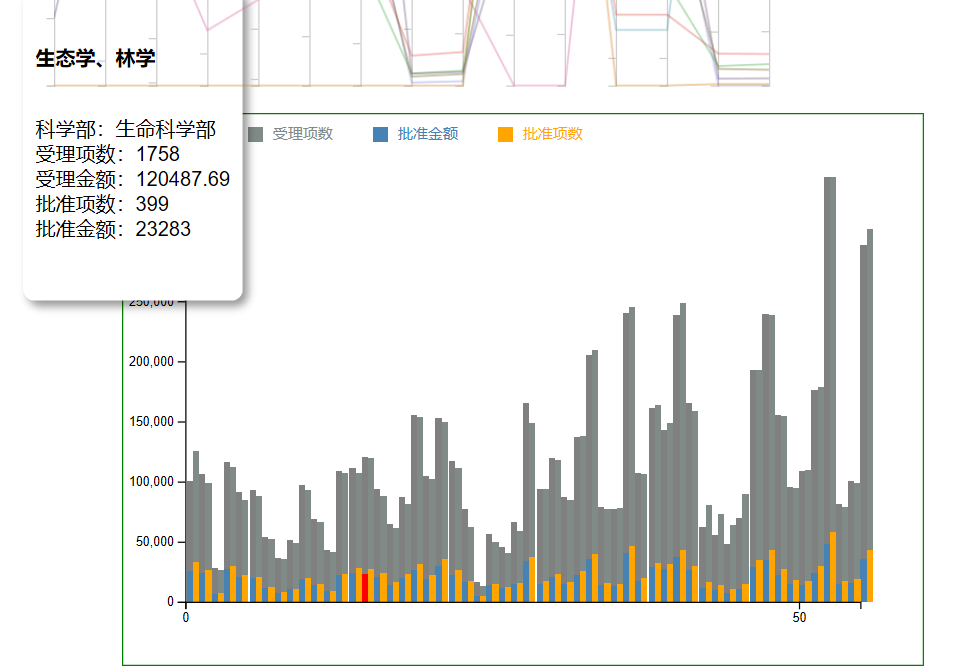
\includegraphics[scale=0.3]{QQ20191028160731.png}
\caption{表单1 以一级学科为分类标准的可视化}
\end{figure}

以一级学科为分类标准,总共有55类,分属于不同的科学部的一级学科之间用白色细线作为间隔划分开来。由于类别数目太多,无法在横轴上标出每个一级学科的名称,也无法在柱状图上直接标出精确数值,因此引入交互标签。将鼠标移到对应的矩形上,会在标签中展示出该类别的具体信息,包括一级学科名、所属科学部、项数、金额。从该图中可以看出,在同一个学部内,不同学科的申请、批准情况的差异也是十分巨大的。

\subsection{表单2}

\begin{figure}[h]
\centering
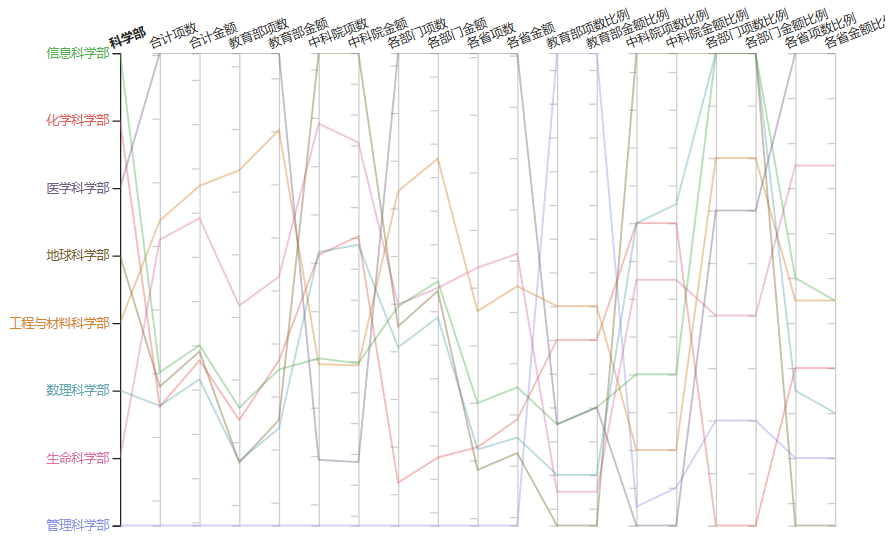
\includegraphics[scale=0.35]{QQ20191028161736.png}
\caption{表单2的可视化}
\end{figure}

将鼠标移到对应坐标轴上,可以看到该坐标轴对应的刻度,并且支持在坐标轴上拖动选区,以提取部分科学部的数据。从该图中,我们可以看出管理科学部的资助主要来自教育部,数理科学部、信息科学部、地球科学部的资助中,来自工、交、农、医、国防等部门的资助比例要比其他的学部高,医学科学部的资助来自各省市自治区的比例比较高。事实上,数理、信息、地球科学等领域在各生产部门之中的应用要比其他学部更为直接、广泛,而医学发展则受到各地政府较大力度的扶持。

\subsection{表单3}

\begin{figure}[h]
\centering
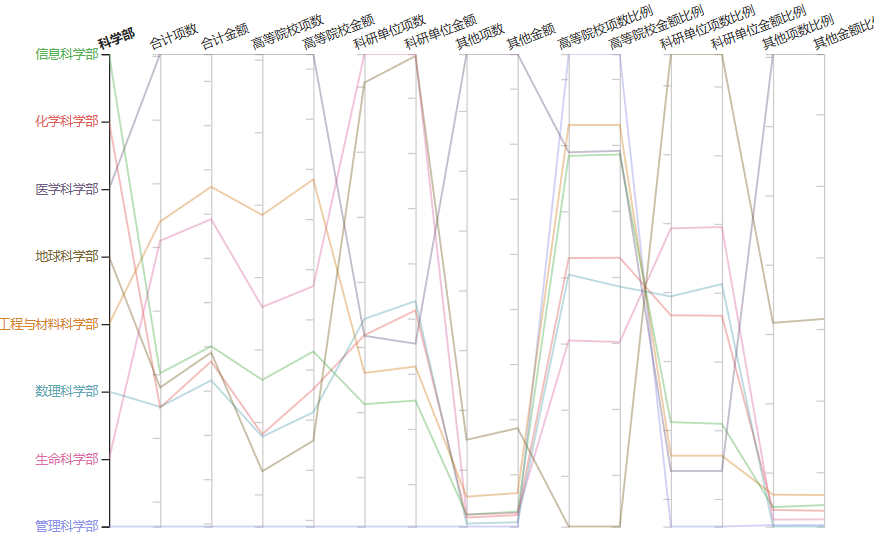
\includegraphics[scale=0.35]{QQ20191028162805.png}
\caption{表单3的可视化}
\end{figure}

与表单2类似,将鼠标移到对应坐标轴上,可以看到该坐标轴对应的刻度,并且支持在坐标轴上拖动选区,以提取部分科学部的数据。从该图中,我们可以看出管理、信息、工程、医学科学部的资助中,高等院校项目所占的比例尤其高,地球科学、生命科学部的资助中科研单位项目所占比例高于其他科学部,其他性质单位的项目资助除了医学科学部外,其他科学部的资助几乎可以忽略不计。高等院校仍然是各学部资助项目申请、研究的主阵地,除了医学可以由医院的研究部门推进科研外,其他学部的科研活动主要还是集中在高等院校和科研单位,这也是符合常识的。

\section{总结与感受}

目前为止,如果我们粗略地使用资助项目的申请、批准情况来推测各学部的发展状况的话,各个学部之间的发展还是相当不平衡的,当然这与学科本身科研经费的消耗是有关的,并受市场调节。此外,各种项目主要是由隶属于教育部、中科院的各个高等院校、科研单位推进的,这充分说明了学术研究项目与工业界之间是有很大区别的。

从可视化实现的过程上看,选用合适的方法对数据进行可视化实现是一件需要技巧、难度较大的工作,需要有较强的理论、实践基础才能比较好地完成。

\end{document}
